% Options for packages loaded elsewhere
\PassOptionsToPackage{unicode}{hyperref}
\PassOptionsToPackage{hyphens}{url}
%
\documentclass[
]{article}
\usepackage{lmodern}
\usepackage{amssymb,amsmath}
\usepackage{ifxetex,ifluatex}
\ifnum 0\ifxetex 1\fi\ifluatex 1\fi=0 % if pdftex
  \usepackage[T1]{fontenc}
  \usepackage[utf8]{inputenc}
  \usepackage{textcomp} % provide euro and other symbols
\else % if luatex or xetex
  \usepackage{unicode-math}
  \defaultfontfeatures{Scale=MatchLowercase}
  \defaultfontfeatures[\rmfamily]{Ligatures=TeX,Scale=1}
\fi
% Use upquote if available, for straight quotes in verbatim environments
\IfFileExists{upquote.sty}{\usepackage{upquote}}{}
\IfFileExists{microtype.sty}{% use microtype if available
  \usepackage[]{microtype}
  \UseMicrotypeSet[protrusion]{basicmath} % disable protrusion for tt fonts
}{}
\makeatletter
\@ifundefined{KOMAClassName}{% if non-KOMA class
  \IfFileExists{parskip.sty}{%
    \usepackage{parskip}
  }{% else
    \setlength{\parindent}{0pt}
    \setlength{\parskip}{6pt plus 2pt minus 1pt}}
}{% if KOMA class
  \KOMAoptions{parskip=half}}
\makeatother
\usepackage{xcolor}
\IfFileExists{xurl.sty}{\usepackage{xurl}}{} % add URL line breaks if available
\IfFileExists{bookmark.sty}{\usepackage{bookmark}}{\usepackage{hyperref}}
\hypersetup{
  pdftitle={Sex-Specific Evolution of the Meiotic Recombination Rate},
  pdfauthor={April L. Peterson, Bret A. Payseur},
  hidelinks,
  pdfcreator={LaTeX via pandoc}}
\urlstyle{same} % disable monospaced font for URLs
\usepackage[margin=1in]{geometry}
\usepackage{graphicx,grffile}
\makeatletter
\def\maxwidth{\ifdim\Gin@nat@width>\linewidth\linewidth\else\Gin@nat@width\fi}
\def\maxheight{\ifdim\Gin@nat@height>\textheight\textheight\else\Gin@nat@height\fi}
\makeatother
% Scale images if necessary, so that they will not overflow the page
% margins by default, and it is still possible to overwrite the defaults
% using explicit options in \includegraphics[width, height, ...]{}
\setkeys{Gin}{width=\maxwidth,height=\maxheight,keepaspectratio}
% Set default figure placement to htbp
\makeatletter
\def\fps@figure{htbp}
\makeatother
\setlength{\emergencystretch}{3em} % prevent overfull lines
\providecommand{\tightlist}{%
  \setlength{\itemsep}{0pt}\setlength{\parskip}{0pt}}
\setcounter{secnumdepth}{-\maxdimen} % remove section numbering
\usepackage{setspace}
\doublespacing
\usepackage{lineno}
\linenumbers
\usepackage{booktabs}
\usepackage{longtable}
\usepackage{array}
\usepackage{multirow}
\usepackage{wrapfig}
\usepackage{float}
\usepackage{colortbl}
\usepackage{pdflscape}
\usepackage{tabu}
\usepackage{threeparttable}
\usepackage{threeparttablex}
\usepackage[normalem]{ulem}
\usepackage{makecell}
\usepackage{xcolor}

\title{Sex-Specific Evolution of the Meiotic Recombination Rate}
\author{April L. Peterson, Bret A. Payseur}
\date{2020-07-29}

\begin{document}
\maketitle

\hypertarget{abstract}{%
\section{ABSTRACT}\label{abstract}}

Although meiotic recombination is required for successful gametogenesis
in most species that reproduce sexually, the rate of crossing over
varies among individuals. Differences in recombination rate between
females and males are perhaps the most striking form of this variation.
Despite the recognition that the sexes recombine at different rates,
existing data fail to address the extent to which recombination
experiences similar evolutionary pressures in the two sexes. To fill
this gap, we measured the genome-wide recombination rate in both sexes
from a panel of wild-derived inbred strains sampled from across three
subspecies of house mice. We applied single-cell immunohistochemistry to
inbred strains to directly compare females and males from the same
genetic background and meiotic context, thereby isolating the effect of
sex on evolutionary differences in recombination. Our results reveal
highly discordant evolutionary trajectories in the two sexes. Whereas
male recombination rates show rapid evolution over short timescales,
female recombination rates measured in the same strains are mostly
static. Strains with high recombination in males have more double-strand
breaks and stronger crossover interference than strains with low
recombination in males, suggesting that these factors contribute to the
sex-specific evolution we document. These results provide the strongest
evidence yet that sex is a primary driver of recombination rate
evolution.

\hypertarget{introduction}{%
\section{INTRODUCTION}\label{introduction}}

Meiosis converts diploid germ cells into haploid gametes. During meiosis
I, DNA crossovers aid the separation of homologous chromosomes by
physically linking them and establishing tension between them on the
spindle (Petronczki et al., 2003). The wrong number of recombination
events can disrupt chromosomal segregation, leading to infertility,
miscarriage, and birth defects (Hassold and Hunt, 2001). Recombination
also shapes evolution by shuffling the combinations of genetic variants
offspring inherit. Recombination affects the fates of beneficial and
deleterious mutations (Felsenstein, 1974; Fisher, 1930; Hill and
Robertson, 1966) and interacts with natural selection to leave gradients
in genomic patterns of diversity (Begun and Aquadro, 1992; Charlesworth
et al., 1993; Cutter and Payseur, 2013; Nachman and Payseur, 2012; Smith
and Haigh, 1974).

The role of recombination in facilitating meiotic chromosome assortment
suggests that the total number of crossovers in a cell -- the
genome-wide recombination rate -- is an important cellular
characteristic connected to organismal fitness. The dual pressures of
ensuring at least one crossover per chromosome and minimizing levels of
DNA damage and ectopic exchange are thought to impose lower and upper
thresholds on the genome-wide recombination rate (Inoue and Lupski,
2002; Nagaoka et al., 2012). Yet, within these bounds, individuals from
the same species can vary substantially in crossover number (Gruhn et
al., 2013; Johnston et al., 2016; Kong et al., 2008; Ma et al., 2015).

Sex is perhaps the most notable axis along which recombination rate
varies. Broadly speaking, sexual dimorphism in the genome-wide
recombination rate assumes two forms. In species such as
\emph{Drosophila melanogaster}, one sex completes meiosis without
forming crossovers (``achiasmy''), while the other sex recombines (Burt
et al., 1991; Haldane, 1922; Huxley, 1928). Alternatively, in most
species with recombination, crossovers occur in both sexes but at
different rates (``heterochiasmy''). In these species, females tend to
recombine more than males (Bell, 1982; Brandvain and Coop, 2012; Burt et
al., 1991; Lenormand and Dutheil, 2005; Lorch, 2005). In plants,
heterochiasmy is correlated with the opportunity for haploid selection
(Lenormand and Dutheil, 2005). Despite the establishment of these
interspecific trends, an understanding of how sex shapes the evolution
of recombination cannot be achieved with available data.

Comprehensive comparisons of variation in female and male recombination
rates within species have come from outbred populations of humans (Gruhn
et al., 2013; Halldorsson et al., 2019; Kong et al., 2004, 2014, 2008),
dog (Campbell et al., 2016), cattle (Ma et al., 2015; Shen et al.,
2018), and Soay sheep (Johnston et al., 2016), in which the role of sex
is confounded with the contributions of genetic variation. Although it
is known that the level and direction of heterochiasmy can differ among
species (Brandvain and Coop, 2012; Lenormand and Dutheil, 2005), the
correlation between female and male recombination rates among closely
related species remains poorly documented. Direct contrasts between the
two sexes across a common, diverse set of genomic backgrounds that
represent recent timescales would reveal whether the genome-wide
recombination rate evolves differently in males and females.

Examining variation in the total number of crossovers in a sex-specific
manner could also illuminate evolutionary connections between
recombination rate and crossover positioning. Analyses of meiotic
chromosome morphology in \emph{Arabidopsis thaliana},
\emph{Caenorhabditis elegans}, and \emph{Mus musculus} suggest that the
sex with more recombination usually has longer chromosome axes (Cahoon
and Libuda, 2019). A survey of 51 species found conserved sex
differences in the recombination landscape, including telomere-biased
placement of crossovers in males but not in females (Sardell and
Kirkpatrick, 2020). The degree to which a crossover reduces the
probability of another crossover nearby (crossover interference) also
differs between females and males (Otto and Payseur, 2019).

The house mouse, \emph{Mus musculus}, is a compelling system for
understanding how sex affects the evolution of recombination. Multiple
subspecies share a most recent common ancestor approximately 0.5 million
years ago (Geraldes et al., 2011), providing the opportunity to examine
natural variation on recent evolutionary timescales. Wild \emph{Mus
musculus} belong to the same species as classical inbred strains of
mice, where the molecular and cellular pathways that lead to crossovers
have been studied extensively (Baudat et al., 2013; Bolcun-Filas and
Schimenti, 2012; Handel and Schimenti, 2010). Single-cell
immunofluorescent approaches make it possible to estimate genome-wide
recombination rates in individual males and females (Koehler et al.,
2002; Peters et al., 1997). A collection of wild-derived inbred strains
founded from a variety of geographic locations is available, enabling
genetic variation in recombination to be profiled across the species
range. Most importantly, by measuring recombination rates in females and
males from the same set of wild-derived inbred strains, the evolutionary
dynamics of recombination can be directly compared in the two sexes.

In this paper, we report genome-wide recombination rates from both sexes
in a diverse panel of wild-derived inbred strains of house mice and
their close relatives. We demonstrate that recombination rate evolves
differently in females and males, even over short timescales.

\begin{figure}
\centering
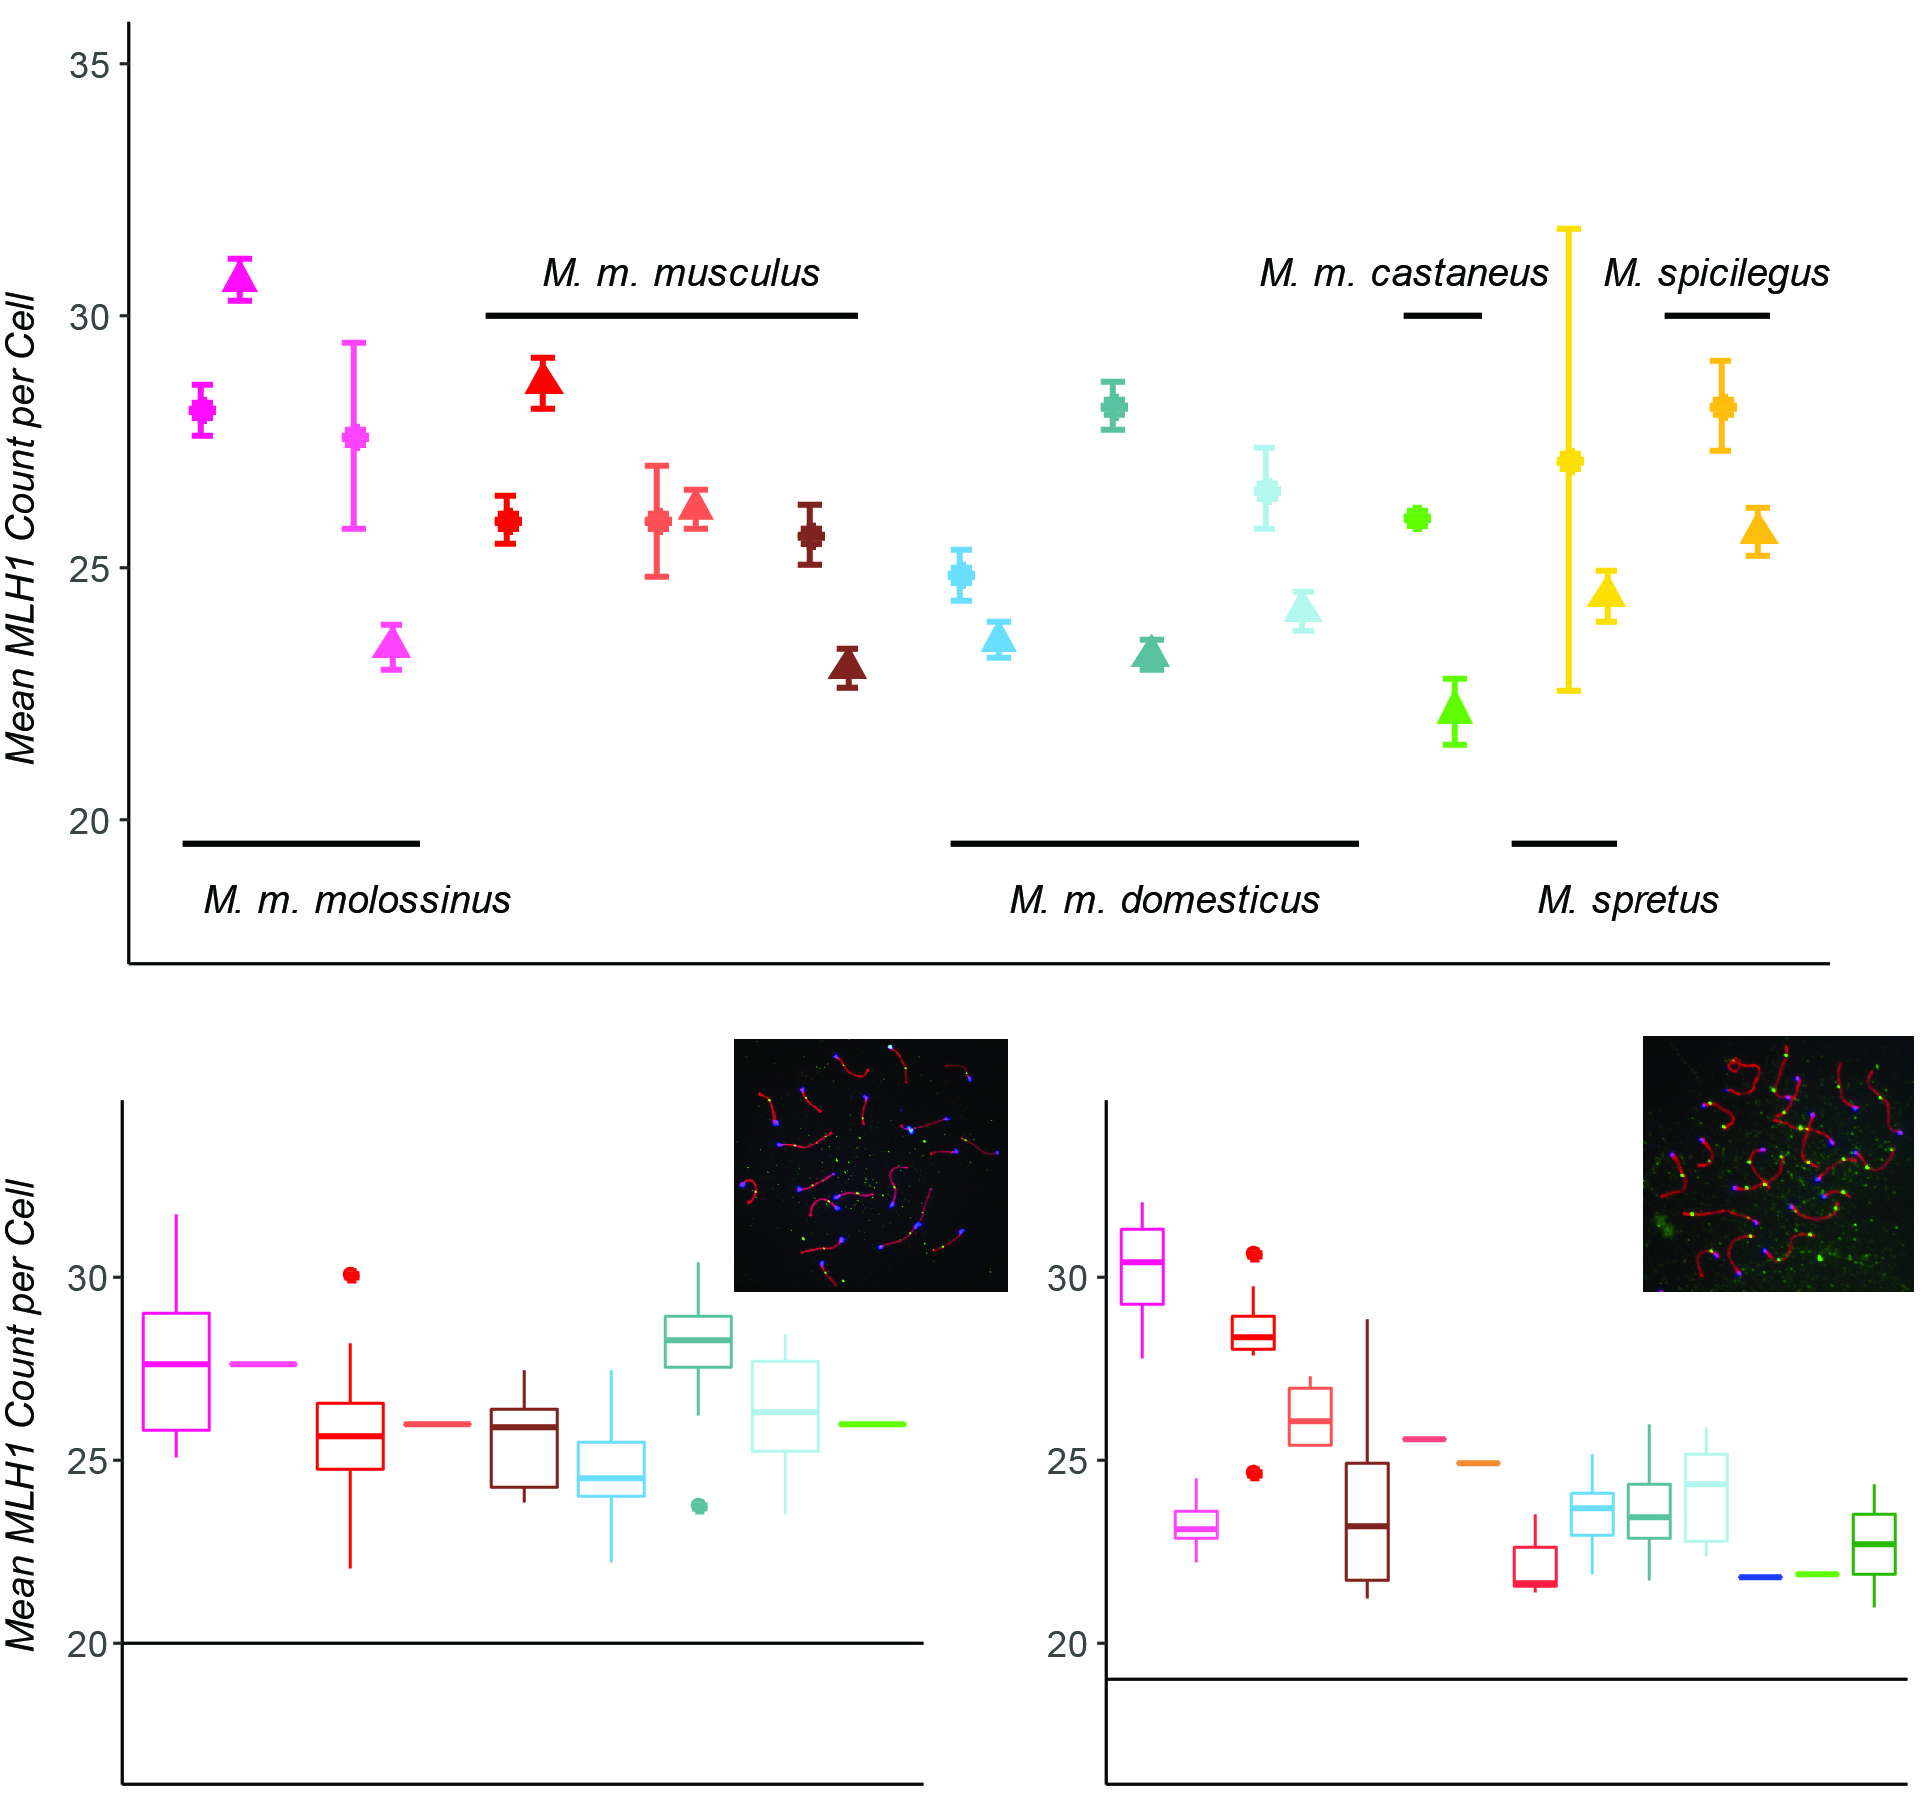
\includegraphics[width=0.5\textwidth,height=\textheight]{Figure1.jpg}
\caption{Caption for the picture.}
\end{figure}

\hypertarget{materials-and-methods}{%
\section{MATERIALS AND METHODS}\label{materials-and-methods}}

\hypertarget{mice}{%
\subsubsection{Mice}\label{mice}}

We used a panel of wild-derived inbred strains of house mice (\emph{Mus
musculus}) and related murid species to profile natural genetic
variation in recombination (Table 4). Mice from the same inbred strain
served as serve as a biological replicates. Our survey included 5
strains from \emph{M. m. musculus}, 4 strains from \emph{M. m.
domesticus}, 2 strains from \emph{M. m. molossinus}, 2 strains from
\emph{M. m. castaneus}, and 1 strain each from \emph{M. spicilegus},
\emph{M. spretus} and \emph{M. caroli}. We subsequently denote strains
by their abbreviated subspecies and name
(\emph{e.g.~domesticus\textsuperscript{WSB}}). Mice were housed at
dedicated, temperature-controlled facilities in the UW-Madison School of
Medicine and Public Health, with the exception of mice from Gough
Island, which were housed in a temperature-controlled facility in the
UW-Madison School of Veterinary Medicine. Mice were sampled from a
partially inbred strain of Gough Island mice, approximately 6
generations of brother-sister matting. All mice were provided with
\emph{ad libitum} food and water. Procedures followed protocols approved
by IACUC.

\hypertarget{tissue-collection-and-immunohistochemistry}{%
\subsubsection{Tissue Collection and
Immunohistochemistry}\label{tissue-collection-and-immunohistochemistry}}

The same dry-down spread technique was applied to both spermatocytes and
oocytes, following Peters et al. (1997), with adjustment for volumes.
Spermatocyte spreads were collected and prepared as described in
Peterson et al. (2019). The majority of mice used for MLH1 counts were
between 5 and 12 weeks of age. Juvenile males between 12 and 15 days of
age were used for DMC1 counts. Both ovaries were collected from embryos
(16-21 embryonic days) or neonates (0-48 hours after birth). Whole
testes were incubated in 3ml of hypotonic solution for 45 minutes.
Decapsulated ovaries were incubated in 300ul of hypotonic solution for
45 minutes. Fifteen microliters of cell slurry (masticated gonads) were
transferred to 80ul of 2\% PFA solution. Cells were fixed in this
solution and dried in a humid chamber at room temperature overnight. The
following morning, slides were treated with a Photoflow wash (Kodak,
diluted 1:200). Slides were stored at -20*C if not stained immediately.
To visualize the structure of meiotic chromosomes, we used antibody
markers for the centromere (CREST) and lateral element of the
synaptonemal complex (SC) (SYCP3). Crossovers (COs) were visualized as
MLH1 foci. Double strand breaks (DSBs) were visualized as DMC1 foci. The
staining protocol followed (Anderson et al., 1999) and (Koehler et al.,
2002). Antibody staining and slide blocking were performed in 1X
antibody dilution buffer (ADB) (normal donkey serum (Jackson
ImmunoResearch), 1X PBS, bovine serum albumin (Sigma), and Triton X-100
(Sigma)). Following a 30-minute blocking wash in ABD, each slide was
incubated with 60ul of a primary antibody master mix for 48 hours at
37*C. The master mix recipe contained polyclonal anti-rabbit anti-MLH1
(Calbiochem; diluted 1:50) or anti-rabbit anti-DMC1 (mix of DMC1),
anti-goat polyclonal anti-SYCP3, (Abcam; diluted 1:50), and anti-human
polyclonal antibody to CREST (Antibodies, Inc; diluted 1:200) suspended
in ADB. Slides were washed twice in 50ml ADB before the first round of
secondary antibody incubation for 12 hours at 37*C. Alexa Fluor 488
donkey anti-rabbit IgG (Invitrgoen, location; diluted to 1:100) and
Coumarin AMCA donkey anti-human IgG (Jackson ImmunoResearch; diluted to
1:200) were suspended in ADB. The last incubation of Alexa Fluor 568
donkey anti-goat (Invitrogen; diluted 1:100) was incubated at 1:100 for
2 hours at 37* C. Slides were fixed with Prolong Gold Antifade
(Invitrogen) for 24 hours after a final wash in 1x PBS. Three slides of
cell spreads per mouse were prepared to serve as technical replicates
for the staining protocol. Comparisons of multiple stained slides from
the same mouse showed no difference in mean MLH1 cell counts and mean
cell quality. Sampled numbers of mice and cells per mouse were maximized
to the extent possible given constraints on breeding and time.

\hypertarget{image-processing}{%
\subsubsection{Image Processing}\label{image-processing}}

Images were captured using a Zeiss Axioplan 2 microscope with AxioLab
camera and AxioVision software (Zeiss, Cambridge, UK). The number of
cells imaged per individual mouse is based on previous studies (Dumont
and Payseur, 2011; Murdoch et al., 2010; Wang and Payseur, 2017).
Preprocessing, including cropping, noise reduction, and histogram
adjustments, was performed using Photoshop (v13.0). Image file names
were anonymized before manual scoring of MLH1 foci or DMC1 foci using
Photoshop.

\hypertarget{analyses}{%
\subsubsection{Analyses}\label{analyses}}

To estimate the number of crossovers across the genome, we counted MLH1
foci within bivalents, synapsed homologous chromosomes. MLH1 foci were
counted in pachytene cells with intact and complete karyotypes (19
acrocentric bivalents and XY for spermatocytes; 20 acrocentric bivalents
for oocytes) and distinct MLH1 foci. A quality score ranging from 1
(best) to 5 (worst) was assigned to each cell based on visual appearance
of staining and spread of bivalents. Cells with a score of 5 were
excluded from the final analysis. Distributions of MLH1 count per cell
were visually inspected for normality (Supplemental Figure 1). When
outliers for MLH1 count were found during preliminary analysis, the
original images were inspected and the counts confirmed.

MLH1 foci located on the XY in spermatocytes were excluded from counts.
In addition to MLH1 counts, we measured several traits to further
characterize the recombination landscape. To estimate the number of
double-strand breaks, a minority of which lead to crossovers, mean DMC1
foci per cell was quantified for a single male from each of a subset of
strains (\emph{molossinus\textsuperscript{MSM}},
\emph{musculus\textsuperscript{PWD}},
\emph{domesticus\textsuperscript{WSB}}, and
\emph{domesticus\textsuperscript{G}} ). SC morphology and CREST foci
number were used to stage spermatocytes as early zygotene or late
zygotene.

To measure bivalent SC length, two image analysis algorithms were used.
The first algorithm estimates the total (summed) SC length across
bivalents for individual cells (Wang et al., 2019). The second algorithm
estimates the SC length of individual bivalents (Peterson et al., 2019).
Both algorithms apply a `skeletonizing' transformation to synapsed
chromosomes that produces a single, pixel-wide `trace' of the bivalent
shape. Total SC length per cell was quantified from pachytene cell
images (Wang et al., 2019).

To reduce algorithmic errors in SC isolation, outliers were visually
identified at the mouse level and removed from the data set. Mouse
averages were calculated from cell-wide total SC lengths in 3,195 out of
3,871 cells with MLH1 counts. SC length of individual bivalents was
quantified in pachytene cell images (Peterson et al., 2019). The DNA
CrossOver algorithm (Peterson et al., 2019) isolates single,
straightened bivalent shapes, returning SC length, location of MLH1
foci, and location of CREST (centromere) foci. The algorithm
substantially speeds the accurate measurement of bivalents, but it
sometimes interprets overlapping bivalents as single bivalents. In our
data set, average proportions of bivalents per cell isolated by the
algorithm ranged from 0.48 (\emph{molossinus\textsuperscript{MSM}} male)
to 0.72 (\emph{musculus\textsuperscript{KAZ}} female). From the total
set of pachytene cell images, 10,213 bivalent objects were isolated by
the algorithm. Following a manual curation, 9,569 single-bivalent
observations remained. The accuracy of the algorithm is high compared to
hand measures after this curation step (Peterson et al., 2019). The
curated single bivalent data supplemented our cell-wide MLH1 count data
with MLH1 foci counts for single bivalents. Proportions of bivalents
with the same number of MLH1 foci were compared across strains using a
chi-square test.

To account for confounding effects of sex chromosomes from pooled
samples of bivalents, we also considered a reduced data set including
only bivalents with SC lengths below the 2nd quartile in cells with at
least 17 of 20 single bivalent measures. This ``short bivalent'' data
set included the four or five shortest bivalents within a cell, thus
excluding the X bivalent in oocytes. A total of 699 short bivalents were
isolated from 102 oocytes and 42 spermatocytes. Although this smaller
data set had decreased power, it offered a more comparable set of single
bivalents to compare between the sexes. A ``long bivalent'' data set was
formed from those bivalents above the 4th quartile in SC lengths per
cell. A total of 703 long bivalents were isolated from 102 oocytes and
42 spermatocytes.

To examine crossover interference, the distance (in SC units) between
MLH1 foci (inter-focal distance; IFD\textsubscript{raw}) was measured
for those single bivalents containing two MLH1 foci. A normalized
measure of interference (IFD\textsubscript{norm}) was computed by
dividing IFD\textsubscript{raw} by SC length on a per-bivalent basis.

We used a series of statistical models to interpret patterns of
variation in the recombination traits we measured (Table 2). We used
mouse average as the dependent variable in all analyses. We first
constructed a linear mixed model (M1) using lmer() from the lmer4
package (Bates et al., 2015) in R (v3.5.2) (Team, 2015). In this model,
strain was coded as a random effect, with significance evaluated using a
likelihood ratio test using exactRLRT() from RLRsim (Scheipl et al.,
2008). Subspecies, sex, and their interaction were coded as fixed
effects, with significance evaluated using a chi-square test comparing
the full and reduced models (drop1() and anova()) (Bates et al., 2015).
The hierarchical nature of the data, meant that nesting of levels across
observations was implicit (\emph{i.e.} mouse within strain, within
subspecies) and not explicitly coded. We used the subspecies effect to
quantify divergence between subspecies and the (random) strain effect to
quantify variation within subspecies in a sex-specific manner. In
separate analyses using model M1, we considered mouse averages as
dependent variables for each of the following traits: MLH1 count per
cell, total SC length per cell, single bivalent SC length per cell,
IFD\textsubscript{raw}, IFD\textsubscript{norm}, and average MLH1
position (for single-focus bivalents). Four additional linear models
containing only fixed effects (M2-M5) (Table 2) were used to further
investigate results obtained from model M1.

\hypertarget{results}{%
\section{RESULTS}\label{results}}

\hypertarget{genome-wide-recombination-rate-evolves-differently-in-females-and-males}{%
\subsection{Genome-wide recombination rate evolves differently in
females and
males}\label{genome-wide-recombination-rate-evolves-differently-in-females-and-males}}

We used counts of MLH1 foci per cell to estimate genome-wide
recombination rates in 14 wild-derived inbred strains sampled from three
subspecies of house mice ( \emph{M. musculus domesticus}, \emph{M. m.
musculus} and \emph{M. m. molossinus} ) and three other species of Mus (
\emph{M. spretus}, \emph{M. spicilegus} , and \emph{M. caroli} ). Mean
MLH1 focus counts for 188 mice were quantified from an average of 21.77
spermatocytes per male (for a total of 1,742 spermatocytes) and 17.85
oocytes per female (for a total of 1,427 oocytes) (Table 1).

Graphical comparisons reveal sex-specific dynamics to the evolution of
genome-wide recombination rate (Figure 1A). First, MLH1 focus counts
differ between females and males in most strains. Second, the difference
in counts between the sexes varies among strains. Although most strains
show more MLH1 foci in females, two strains
(\emph{musculus\textsuperscript{PWD}} and
\emph{molossinus\textsuperscript{MSM}}) exhibit higher counts in males.
In females, numbers of MLH1 foci are evenly distributed around the
sex-wide mean of approximately 25 (Figure 1B). In stark contrast, males
largely separate into two groups of strains with high numbers (near 30)
and low numbers (near 23) of foci (Figure 1C). Strain mean MLH1 focus
counts from females and males are uncorrelated (Spearman's \(\rho\) =
0.08; p = 0.84) across the set of strains.

\begin{table}[H]
\centering
\resizebox{\linewidth}{!}{
\begin{tabular}{l|l|l|l|l|l|l|l|l|l}
\hline
Species & Subspecies & Strain & Sex & Number.of.Mice & Number.of..Cells & Mean.MLH1.Count & SE & cV & Variance\\
\hline
M. musculus & M. m. domesticus & WSB & female & 14 & 184 & 24.701 & 0.267 & 14.638271224837814 & 13.074\\
\cline{1-10}
 &  &  & male & 11 & 222 & 23.383 & 0.18 & 11.479933887268658 & 7.206\\
\cline{3-10}
 &  & G & female & 12 & 318 & 28.211 & 0.235 & 14.835969061582837 & 17.517\\
\cline{3-10}
 &  &  & male & 18 & 355 & 23.161 & 0.14 & 11.35380583435758 & 6.915\\
\cline{3-10}
 &  & LEW & female & 9 & 147 & 26.585 & 0.398 & 18.16189516714001 & 23.313\\
\cline{3-10}
 &  &  & male & 10 & 253 & 24.162 & 0.195 & 12.83701437670674 & 9.62\\
\cline{3-10}
 & \multirow{-6}{*}{\raggedright\arraybackslash } & PERC & male & 1 & 26 & 21.808 & 0.41 & 9.71 & 4.48\\
\cline{2-10}
 & M. m. musculus & PWD & female & 15 & 222 & 25.977 & 0.251 & 14.41018621027294 & 14.013\\
\cline{2-10}
 &  &  & male & 8 & 161 & 28.671 & 0.246 & 10.896284161204306 & 9.76\\
\cline{3-10}
 &  & SKIVE & female & 1 & 32 & 25.938 & 0.553 & 12.070868672504577 & 9.802\\
\cline{3-10}
 &  &  & male & 3 & 86 & 26.081 & 0.293 & 10.408689886052935 & 7.37\\
\cline{3-10}
 &  & KAZ & female & 9 & 184 & 25.625 & 0.295 & 15.62873696060005 & 16.039\\
\cline{3-10}
 &  &  & male & 13 & 264 & 22.989 & 0.186 & 13.159636243359548 & 9.152\\
\cline{3-10}
 &  & CZECH & male & 3 & 62 & 22.3 & 0.32 & 11.21 & 6.25\\
\cline{3-10}
 &  & AST & male & 3 & 63 & 24.41 & 0.33 & 10.65 & 6.76\\
\cline{3-10}
 & \multirow{-8}{*}{\raggedright\arraybackslash } & TOM & male & 2 & 10 & 23.7 & 1.18 & 15.79 & 14.01\\
\cline{2-10}
 & M. m. castaneus & CAST & female & 1 & 1 & 26 & NA &  & \\
\cline{2-10}
 &  &  & male & 2 & 44 & 22 & 0.34 & 10 & 5.2\\
\cline{3-10}
 & \multirow{-2}{*}{\raggedright\arraybackslash } & HMI & male & 4 & 44 & 24 & 0.41 & 11 & 7.5\\
\cline{2-10}
 & M. m. molossinus & MSM & female & 14 & 300 & 28.123 & 0.254 & 15.64239374084605 & 19.353\\
\cline{2-10}
 &  &  & male & 7 & 166 & 30.367 & 0.242 & 10.262658213499735 & 9.713\\
\cline{3-10}
 &  & MOLF & female & 1 & 21 & 27.619 & 0.924 & 15.33891788564294 & 17.948\\
\cline{3-10}
\multirow{-22}{*}{\raggedright\arraybackslash } &  &  & male & 6 & 119 & 23.42 & 0.232 & 10.80040516644884 & 6.398\\
\cline{1-1}
\cline{3-10}
Mus spretus &  & SPRET & female & 2 & 2 & 26 & 2 & 10.878565864408424 & 8\\
\cline{1-1}
\cline{3-10}
 &  &  & male & 5 & 103 & 24.427 & 0.246 & 10.232121984584271 & 6.247\\
\cline{1-1}
\cline{3-10}
Mus spicilegus &  & SPIC & female & 6 & 97 & 28.237 & 0.448 & 15.628316890383017 & 19.474\\
\cline{1-1}
\cline{3-10}
 &  &  & male & 4 & 133 & 25.774 & 0.241 & 10.781039022222362 & 7.721\\
\cline{1-1}
\cline{3-10}
Mus caroli & \multirow{-8}{*}{\raggedright\arraybackslash } & CAROLI & male & 2 & 57 & 27 & 0.4 & 11 & 8.9\\
\hline
\end{tabular}}
\end{table}

To further partition variation in recombination rate, we fit a series of
linear models to mean MLH1 focus counts from 137 house mice from three
subspecies; \emph{M. m. domesticus}, \emph{M. m. musculus} and \emph{M.
m. molossinus} (Table 2; detailed results available in Supplemental
Table X). Strain, sex, subspecies, and sex*subspecies each affect MLH1
focus count in a linear mixed model (M1; strain (random effect): p
\textless{} \ensuremath{10^{-4}}-- 10-4; sex: p =
\ensuremath{3.64\times 10^{-6}}; subspecies: p =
\ensuremath{9.69\times 10^{-4}}; subspecies*sex: p =
\ensuremath{1.8\times 10^{-4}}).

The effect of subspecies is no longer significant in a model treating
all factors as fixed effects (M2; \emph{musculus} p = 0.24,
\emph{molossinus} p = 0.1), highlighting strain and sex as salient
variables. Two strains exhibit strong effects on MLH1 focus count (M3;
\emph{domesticus\textsuperscript{G}} p =
\ensuremath{1.78\times 10^{-6}}; \emph{domesticus\textsuperscript{LEW}}
p = 0.02), with sex-strain interactions involving three strains (M3;
\emph{domesticus\textsuperscript{G}} p \textless{} 10-6 -- 0;
\emph{molossinus\textsuperscript{MSM}} p \textless{} 10-6 -- 0;
\emph{musculus\textsuperscript{PWD}} p =
\ensuremath{3.87\times 10^{-4}}). \textbf{fix the pvalue above, change
the 0 to p \textless{} 10\^{}-6}

\begin{figure}
\centering
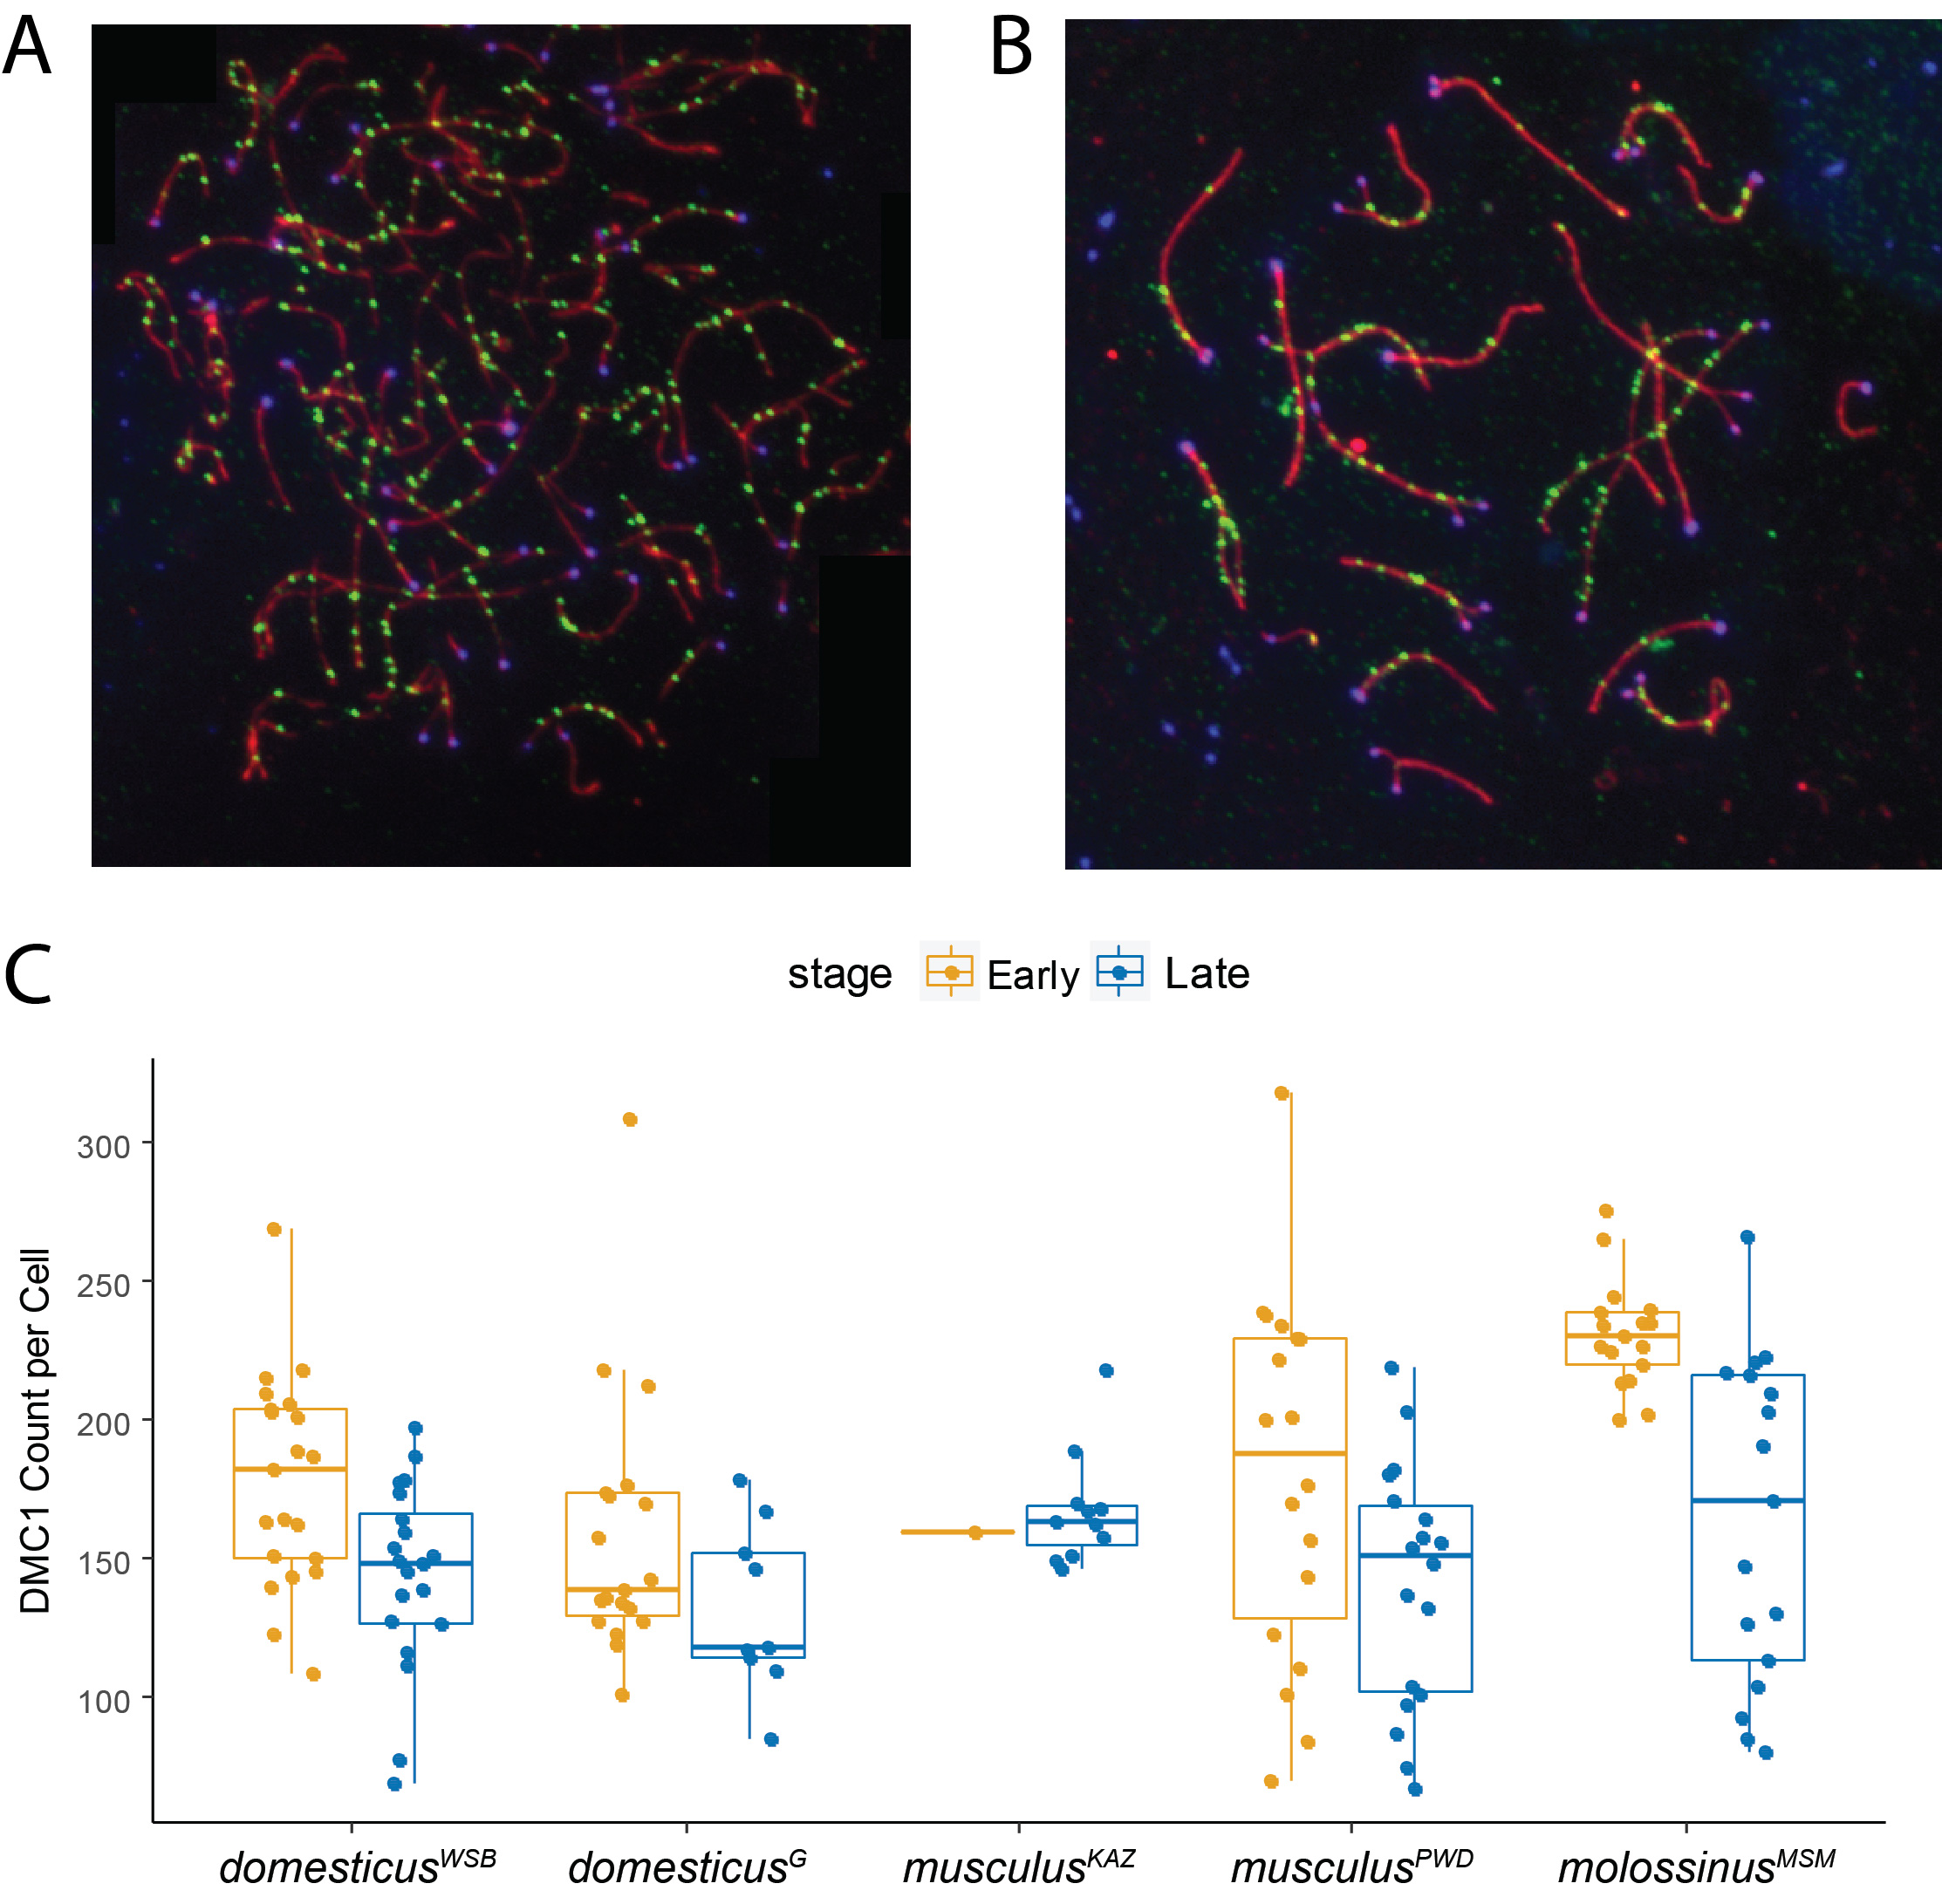
\includegraphics[width=0.5\textwidth,height=\textheight]{Figure2.jpg}
\caption{Caption for the picture.}
\end{figure}

In separate analyses of males (M4; n = 71), three strains
disproportionately shape MLH1 focus count (as observed in Figure 1C):
\emph{musculus\textsuperscript{PWD}} (p =
\ensuremath{3.6\times 10^{-7}}; effect = 6.11 foci,
\emph{molossinus\textsuperscript{MSM}} (p =
\ensuremath{6.3\times 10^{-9}}; effect = 6.91), and
\emph{musculus\textsuperscript{SKIVE}} (p =
\ensuremath{8.22\times 10^{-4}}; effect = 4.04). These three strains
point to substantial evolution in the genome-wide recombination rate in
spermatocytes; we subsequently refer to them as ``high-recombination''
strains. In females (M4; n= 76 ), three strains affect MLH1 focus count:
\emph{domesticus\textsuperscript{G}} (p =
\ensuremath{8.7\times 10^{-6}}; effect = 3.3),
\emph{molossinus\textsuperscript{MSM}} (p =
\ensuremath{2.43\times 10^{-5}}; effect = 2.99), and
\emph{domesticus\textsuperscript{LEW}} (p = 0.03; effect = 1.69). Strain
effect sizes in females are modest in magnitude compared to those in
males. Together, these results demonstrate that the genome-wide
recombination rate evolves in a highly sex-specific manner.

\hypertarget{synaptonemal-complexes-are-longer-in-females}{%
\subsection{Synaptonemal complexes are longer in
females}\label{synaptonemal-complexes-are-longer-in-females}}

The variation in sex differences in recombination we discovered provided
an opportunity to determine whether sex differences in chromatin
compaction, as measured by the length of the synaptonemal complex (SC),
are reversed when heterochiasmy is reversed. In all strains except
\emph{musculus\textsuperscript{SKIVE}}, females have longer SCs than
males, whether SC length was estimated as the total length across
bivalents or as the length of short bivalents (t-tests; all p
\textless{} 0.05, except short bivalents in
\emph{musculus\textsuperscript{SKIVE}}, p = 0.11). Among short bivalents
(to which the female X bivalent does not contribute), female to male
ratios of mouse mean SC length range from 1.26
(\emph{musculus\textsuperscript{PWD}}) to 1.52
(\emph{domesticus\textsuperscript{WSB}}) across strains. That females
have longer SCs is further supported by models that include covariates,
which identify sex as the most consistently significant effect for total
SC length (M1: p = \ensuremath{2.56\times 10^{-31}}; M2: p =
\ensuremath{2.56\times 10^{-8}}; M3: p =
\ensuremath{2.56\times 10^{-8}}) and short bivalent SC length (M1: p =
\ensuremath{1.12\times 10^{-11}}; M2: p \textless{} 0; M3: p \textless{}
0). The existence of some subspecies and strain effects on total SC
length and short bivalent SC length (Supplemental Tables 5 and 8)
further indicates that SC length has evolved among strains and among
subspecies.

In summary, two approaches for measuring SC length demonstrate that
females have longer SCs (chromosome axes), even in strains in which
males recombine more. This pattern implies that in high-recombination
strains, spermatocytes have less space than oocytes in which to position
additional crossovers.

\begin{figure}
\centering
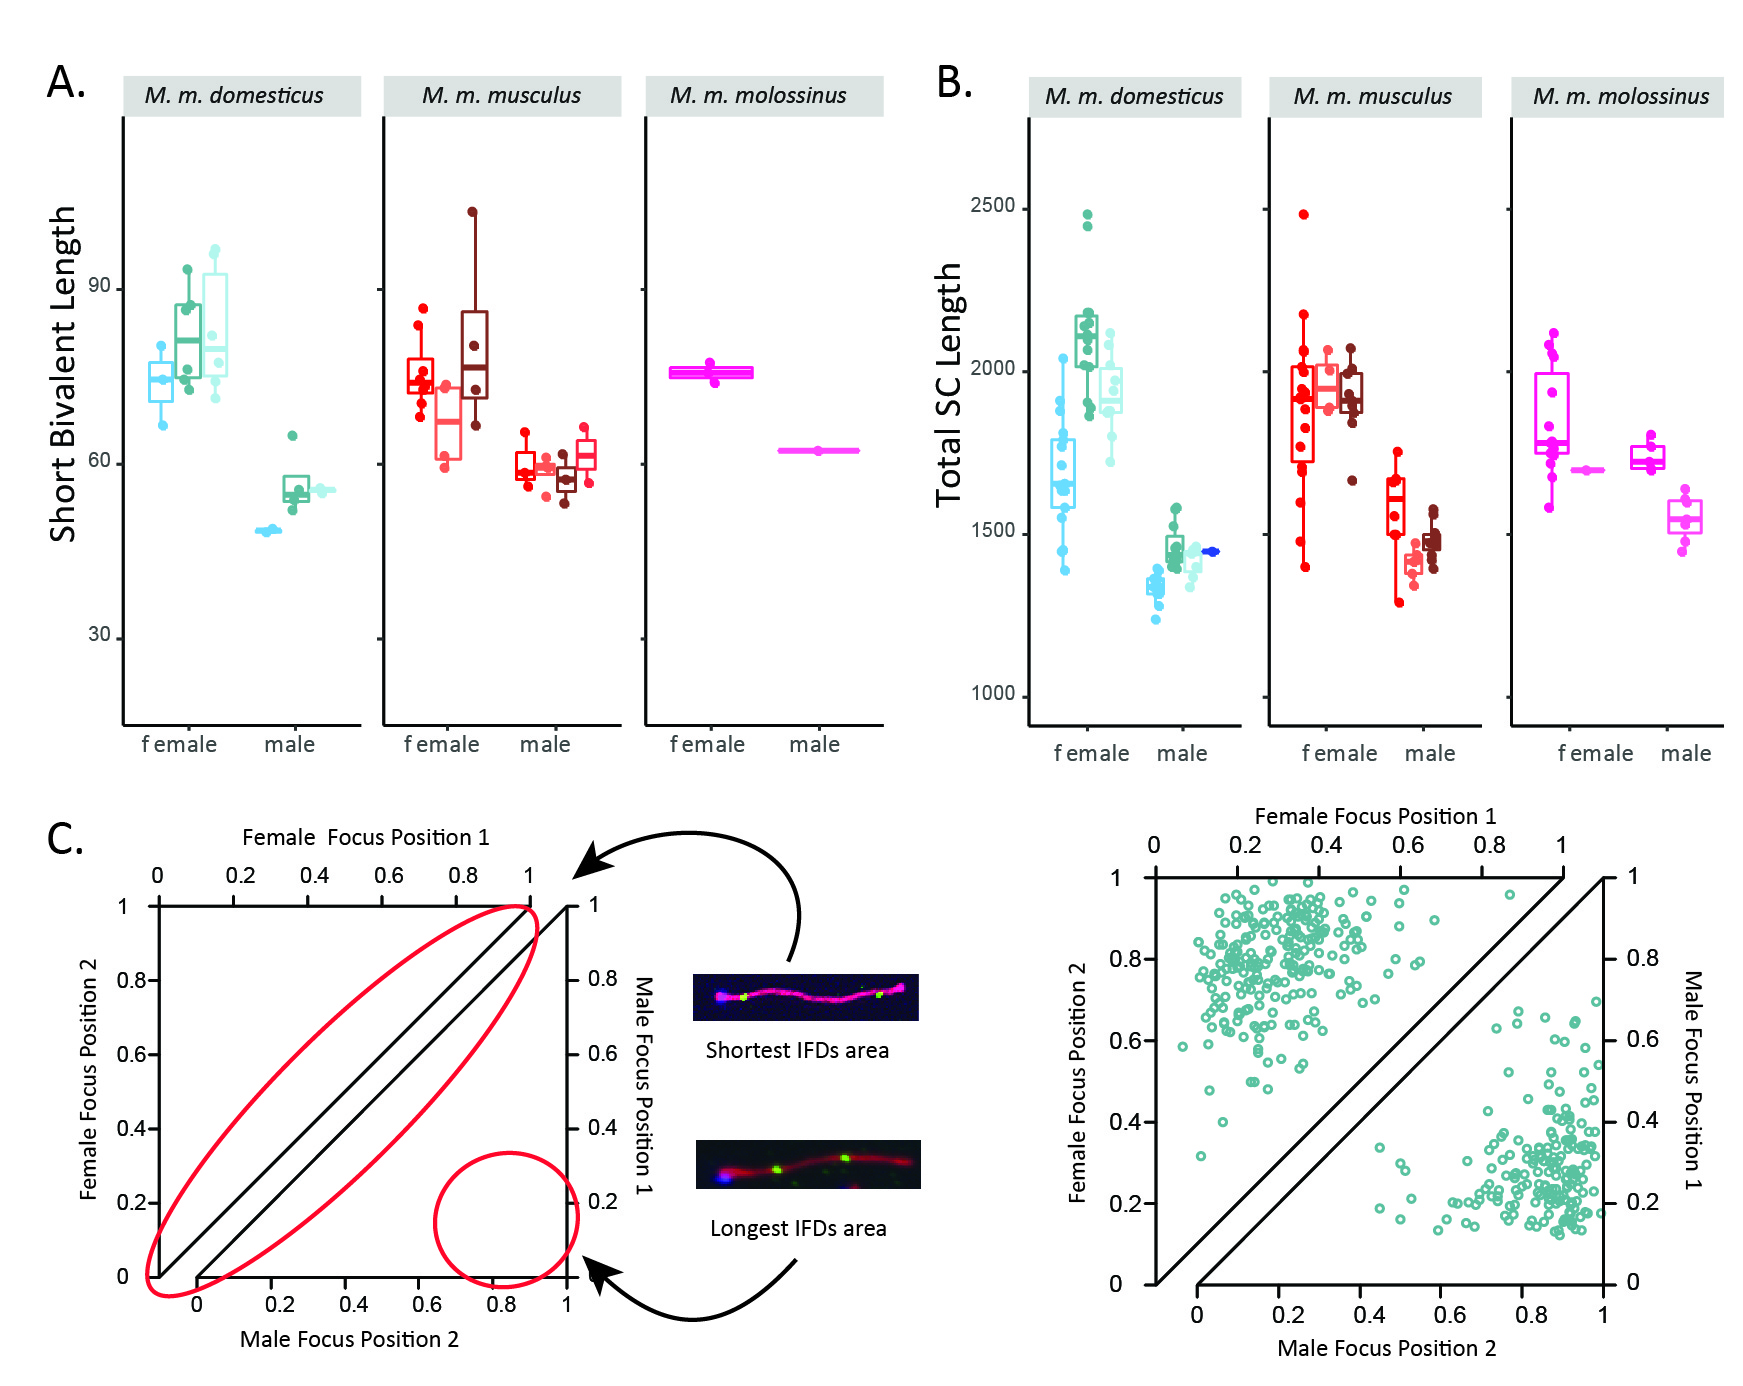
\includegraphics[width=0.5\textwidth,height=\textheight]{Fig3_SC.jpg}
\caption{Caption for the picture.}
\end{figure}

\hypertarget{females-and-males-differ-in-crossover-positions-and-crossover-interference}{%
\subsection{Females and males differ in crossover positions and
crossover
interference}\label{females-and-males-differ-in-crossover-positions-and-crossover-interference}}

We used normalized positions of MLH1 foci along bivalents with a single
focus to compare crossover location while controlling for differences in
SC length. In all strains, MLH1 foci tend to be closer to the telomere
in males (mean normalized position in males: 0.68; mean normalized
position in females: 0.56; paired t-test; p =
\ensuremath{8.49\times 10^{-4}}). Sex is also the strongest determinant
of MLH1 focus position in the models we tested (M1: p =
\ensuremath{2.82\times 10^{-26}}; M2: p =
\ensuremath{3.96\times 10^{-8}}; M3: p =
\ensuremath{3.96\times 10^{-8}}).

Males have longer normalized mean inter-focal distances
(IFD\textsubscript{norm}) than females in seven out of eight strains
(t-tests; p \textless{} 0.05), with only
\emph{musculus\textsuperscript{KAZ}} showing no difference (p = 0.33).
Examination of IFD\textsubscript{norm} distributions indicates that
females are centered at approximately 50\% and show a slight enrichment
of low (\textless25\%) values, whereas males are enriched for higher
values. Models treating IFD\textsubscript{norm} as the dependent
variable support the inference of stronger interference in males, with
sex being the most significant variable (M1: p =
\ensuremath{9.08\times 10^{-12}}; M2: p = 0.01; M3: p = 0.01). In
contrast, there is no clear signal of sex differences in raw mean
inter-focal distances (IFD\textsubscript{raw}) (Supplemental Table 13
and 14) across the full set of strains, whether they are considered
separately or together. Visualization of normalized MLH1 foci positions
on bivalents with two crossovers (Figure 3C and Supplemental Figure 3)
further suggests that interference distances vary more in females than
in males, and that males display a stronger telomeric bias in the
placement of the distal crossover.

In summary, controlling for differences in SC length (chromatin
compaction) indicates that interference is consistently stronger in
males, whereas interference on the physical scale is similar in the two
sexes.

\hypertarget{evolution-of-genome-wide-recombination-rate-is-dispersed-across-bivalents-associated-with-double-strand-break-number-and-connected-to-crossover-interference}{%
\subsection{Evolution of genome-wide recombination rate is dispersed
across bivalents, associated with double-strand break number, and
connected to crossover
interference}\label{evolution-of-genome-wide-recombination-rate-is-dispersed-across-bivalents-associated-with-double-strand-break-number-and-connected-to-crossover-interference}}

We used the contrast between males from high-recombination strains and
males from low-recombination strains to identify features of the
recombination landscape associated with evolutionary transitions in the
genome-wide recombination rate. We considered proportions of bivalents
with different numbers of crossovers, double-strand break number, SC
length, and crossover positioning.

Ninety-six percent of single bivalents in our pooled dataset (n = 9,569)
have either one or two MLH foci (Supplemental Figure 2). The proportions
of single-focus (1CO) bivalents vs.~double-focus (2CO) bivalents
distinguish high-recombination strains from low-recombination strains
(Supplemental Figure 2). High-recombination strains are enriched for 2CO
bivalents at the expense of 1CO bivalents: proportions of 2CO bivalents
are 0.33 in \emph{musculus\textsuperscript{SKIVE}}, 0.44 in
\emph{musculus\textsuperscript{PWD}}, and 0.51 in
\emph{molossinus\textsuperscript{MSM}} (Supplemental Figure 3).
Following patterns in the genome-wide recombination rate, male
\emph{musculus\textsuperscript{PWD}} and male
\emph{molossinus\textsuperscript{MSM}} have 2CO proportions that are
more similar to each other than to strains from their own subspecies
(chi-square tests; \emph{musculus\textsuperscript{PWD}}
vs.~\emph{molossinus\textsuperscript{MSM}}: p = 0.37;
\emph{musculus\textsuperscript{PWD}}
vs.~\emph{musculus\textsuperscript{KAZ}}: p =
\ensuremath{1.23\times 10^{-31}}; \emph{molossinus\textsuperscript{MSM}}
vs.~\emph{molossinus\textsuperscript{MOLF}}: p =
\ensuremath{2.34\times 10^{-6}}). These results demonstrate that
evolution of the genome-wide recombination rate reflects changes in
crossover number across multiple bivalents.

To begin to localize evolution of genome-wide recombination rate to
steps of the recombination pathway, we counted DMC1 foci in prophase
spermatocytes as markers for double-strand breaks (DSBs). DMC1 foci were
counted in a total of 76 early zygotene and 75 late zygotene
spermatocytes from two high-recombination strains
(\emph{musculus\textsuperscript{PWD}} and
\emph{molossinus\textsuperscript{MSM}}) and three low-recombination
strains (\emph{musculus\textsuperscript{KAZ}},
\emph{domesticus\textsuperscript{WSB}}, and
\emph{domesticus\textsuperscript{G}}) (Table 3). High-recombination
strains have significantly more DMC1 foci than low-recombination strains
in early zygotene cells (t-test; p \textless{} \ensuremath{10^{-6}}). In
contrast, the two strain groups do not differ in DMC1 foci in late
zygotene cells (t-test; p = 0.66). Since DSBs are repaired as either COs
or non-crossovers (NCOs), the ratio of MLH1 foci to DMC1 foci can be
used to estimate the proportion of DSBs designated as COs.
High-recombination and low-recombination strains do not differ in the
MLH1/DMC1 ratio, whether DMC1 foci were counted in early zygotene cells
or late zygotene cells (t-test; p \textgreater{} 0.05). These results
raise the possibility that the evolution of genome-wide recombination
rate is primarily determined by processes that precede the CO/NCO
decision, at least in house mice.

Total SC length only partially differentiates high-recombination strains
from low-recombination strains (Figure 3). Whereas high-recombination
strains as a group have significantly greater total SC length than
low-recombination strains (t-test; p = 0.01), separate tests within
subspecies show that the two strain categories differ within \emph{M. m.
molossinus} (p = \ensuremath{2.59\times 10^{-4}}) but not within
\emph{M. m. musculus} (p = 0.65). Additionally, mouse means for the
reduced (short and long) bivalent datasets do not differ between
high-recombination and low-recombination strains (t-test; short: p =
0.84; long: p = 0.19). In a model with total SC length as the dependent
variable (M4), the two subspecies effects are significant (\emph{M. m.
musculus} p = \ensuremath{3.95\times 10^{-7}}; \emph{M. m. molossinus} p
= \ensuremath{3.33\times 10^{-7}}), but there are also strain-specific
effects (Supplemental Table 6). In models with SC lengths of short and
long bivalents as dependent variables, several subspecies and strain
effects reach significance (p \textless{} 0.05) (Supplemental Table 9),
but they are not consistent across models. Collectively, these results
reveal that evolution of SC length is not strongly associated with
evolution of genome-wide recombination rate in house mice.

In summary, evolution of the genome-wide recombination rate in males is
connected to double-strand break number and crossover interference, but
not to SC length and crossover position (on single-crossover bivalents).

\hypertarget{discussion}{%
\section{DISCUSSION}\label{discussion}}

By comparing recombination rates in females and males from the same
diverse set of genetic backgrounds, we isolated sex as a primary factor
in the evolution of this fundamental meiotic trait. Recombination rate
differences are more pronounced in males than females. Because
inter-strain divergence times are identical for the two sexes, this
observation demonstrates that the genome-wide recombination rate evolves
faster in males. More generally, recombination rate divergence is
decoupled in females and males. These disparities are remarkable given
that recombination rates for the two sexes were measured in identical
genomic backgrounds (other than the number and identity of sex
chromosomes). Our results provide the strongest evidence yet that the
genome-wide recombination rate follows distinct evolutionary
trajectories in males and females.

At the genetic level, the sex-specific patterns we documented indicate
that some mutations responsible for the evolution of recombination rate
have dissimilar phenotypic effects in the two sexes. A subset of the
genetic variants associated with genome-wide recombination rate within
populations of humans (Halldorsson et al., 2019; Kong et al., 2004,
2014, 2008), cattle (Ma et al., 2015; Shen et al., 2018), and Soay sheep
(Johnston et al., 2016) appear to show sex-specific properties,
including opposite effects in females and males. Furthermore,
inter-sexual correlations for recombination rate are weak in humans
(Fledel-Alon et al., 2011) and Soay sheep (Johnston et al., 2016).
Crosses between the strains we surveyed could be used to identify and
characterize the genetic variants responsible for recombination rate
evolution in house mice (Dumont and Payseur, 2011; Wang et al., 2019;
Wang and Payseur, 2017). These variants could differentially affect
females and males at any step in the recombination pathway. Although our
DMC1 profiling was limited to males from a small number of strains (for
practical reasons), our findings suggest that mutations that determine
the number of double-strand breaks contribute to sex-specific evolution
in the recombination rate. A study of two classical inbred strains and
one wild-derived inbred strain of house mice also found a positive
association between crossover number and double-strand break number in
males (Baier et al., 2014).

Another implication of our results is that the connection between
recombination rate and fitness differs between males and females. Little
is known about whether and how natural selection shapes recombination
rate in nature (Dapper and Payseur, 2017; Ritz et al., 2017). Samuk et
al. (2020) recently used a quantitative genetic test to conclude that an
8\% difference in genome-wide recombination rate between females from
two populations of\_Drosophila pseudoobscura\_ was caused by natural
selection. Applying similar strategies to species in which both sexes
recombine, including house mice, would be a logical next step to
understanding the sex-specific evolution of recombination rate.

Population genetic models have been built to explain sexual dimorphism
in the number and placement of crossovers, which is a common phenomenon
(Brandvain and Coop, 2012; Sardell and Kirkpatrick, 2020). Modifier
models predicted that lower recombination rates in males will result
from haploid selection (Lenormand, 2003) or sexually antagonistic
selection on coding and cis-regulatory regions of genes (Sardell and
Kirkpatrick, 2020). Another modifier model showed that meiotic drive
could stimulate female-specific evolution of the recombination rate
(Brandvain and Coop, 2012). Although these models fit the conserved
pattern of sex differences in crossover positions, they do not readily
explain our observations of sex-specific evolution in the genome-wide
recombination rate. In particular, the alternation across strains in
which sex has more crossovers is unexpected.

\textless SAC section 1\textgreater{}

We propose an alternative interpretation of our findings based on the
cell biology of gametogenesis. During meiosis, achieving a stable
chromosome structure requires the attachment of kinetochores to opposite
poles of the cell and at least one crossover to create tension across
the sister chromosome cohesion distal to chiasmata (Dumont and Desai,
2012; Lane and Kauppi, 2019; Subramanian and Hochwagen, 2014; VanVeen
and Hawley, 2003). The spindle assembly checkpoint (SAC) prevents
aneuploidy by ensuring that all bivalents are correctly attached to the
microtubule spindle (``bi-oriented'') before starting the
metaphase-to-anaphase transition via the release of the sister cohesion
holding homologs together (Lane and Kauppi, 2019). Hence, selection
seems likely to favor mutations that optimize the process of
bi-orientation and chromosome separation, thereby prohibiting the SAC
from delaying the cell cycle or triggering apoptosis. Multiple lines of
evidence indicate that the SAC is more effective in spermatogenesis than
in oogenesis (Lane and Kauppi, 2019), perhaps due to the presence of the
acentrosome spindle (So et al., 2019) and larger cell volume (Kyogoku
and Kitajima, 2017) in oocytes. The higher stringency of the SAC during
spermatogenesis suggests that selection will be better at removing
mutations that interfere with bi-orientation in males than in females.
Therefore, faster male evolution of the genome-wide recombination rate
could be driven by the more stringent SAC acting on chromosome
structures at the metaphase I alignment.

Our SAC model is consistent with other features of our data. We showed
that widespread sex differences in broad-scale crossover positioning
(Sardell and Kirkpatrick, 2020) apply across house mice, even in
lineages where the direction of heterochiasmy is reversed. Faster
spermatogenesis may select for synchronization of the separation across
all homologs within the cell (Kudo et al., 2009), whereas in oogenesis,
the slower cell cycle and multiple arrest stages may require chromosome
structures with greater stability on the meiosis I spindle, especially
for those organisms that undergo dictyate arrest (Lee, 2019).

We propose that the SAC model also can explain the correlated evolution
of stronger crossover interference and higher genome-wide recombination
rate in male house mice. Our results show that crossovers are spaced
further apart in strains enriched for double-crossover bivalents when SC
length is considered and bivalent size effects are minimized. Assuming
chromatin compaction between (prophase) pachytene and metaphase is
uniform along bivalents, this increased spacing is expected to expand
the area for sister cohesion to connect homologs and may improve the
fidelity of chromosomal segregation. While the SAC model postulates
direct fitness effects of interference, a modifier model predicted that
indirect selection on recombination rate -- via its modulation of
offspring genotypes -- can strengthen interference as well (Goldstein et
al., 1993).

Regardless of the underlying mechanism, our results provide a rare
demonstration that crossover interference can diverge over short
evolutionary timescales. The notion that stronger interference can
co-evolve with higher genome-wide recombination rate is supported by
differences between breeds of cattle (Ma et al., 2015). In contrast,
mammalian species with stronger interference tend to exhibit lower
genome-wide recombination rates (Otto and Payseur, 2019; Segura et al.,
2013). The evolution of crossover interference and its relationship to
changes in crossover number on the genomic scale is a topic deserving of
more empirical and theoretical work. Our findings further reveal that
evolution of the genome-wide recombination rate does not require major
changes in the degree of chromatin compaction. Female house mice
consistently show longer SCs, even in strains with more recombination in
males. Studies in mice (Lynn et al., 2002; Petkov et al., 2007) and
humans (Gruhn et al., 2013; Tease and Hulten, 2004) suggest that
chromosomal axes are longer (and DNA loops are shorter) in females than
males. Some authors have suggested that conserved sex differences in
crossover positioning (more uniform placement in females) and
interference strength (stronger interference in males) could be due to
looser chromatin packing of the meiotic chromosome structure in females
(Haenel et al., 2018; Petkov et al., 2007). A cellular model designed to
explain interference attributes sexual dimorphism in chromatin structure
to greater cell volumes and oscillatory movements of telomeres and
kinetochores in oocytes (Hultén, 2011). Recent work in mice connects the
sparser recombination landscape in females to sex differences in
crossover maturation efficiency (Wang et al., 2017).

Our conclusions are accompanied by several caveats. First, MLH1 foci
only identify interfering crossovers (Holloway et al., 2008). Although
most crossovers belong to this class (Holloway et al., 2008), our
approach likely underestimated genome-wide recombination rates.
Evolution of the number of non-interfering crossovers is a subject worth
examining. A second limitation is that our investigation of crossover
locations was confined to the relatively low resolution possible with
immunofluorescent cytology. Positioning crossovers with higher
resolution could reveal additional evolutionary patterns. Finally, the
panel of inbred lines we surveyed may not be representative of
recombination rate variation within and between subspecies of house
mice. We considered most available wild-derived inbred lines, but house
mice have a broad geographic distribution. Nevertheless, we expect our
primary conclusion that recombination rate evolves in a sex-specific
manner to be robust to geographic sampling because differences between
females and males exist for the same set of inbred strains.

While the causes of sex differences in recombination remain mysterious
Lenormand et al. (2016), our conclusions have implications for a wide
range of recombination research. For biologists uncovering the cellular
and molecular determinants of recombination, our results suggest that
mechanistic differences between the sexes could vary by genetic
background. For researchers charting the evolutionary trajectory of
recombination, our findings indicate that sex-specific comparisons are
crucial. For theoreticians building evolutionary models of
recombination, different fitness regimes and genetic architectures in
females and males should be considered. Elevating sex as a primary
determinant of recombination would be a promising step toward
integrating knowledge of cellular mechanisms with evolutionary patterns
to understand recombination rate variation in nature.

\hypertarget{acknowledgements}{%
\section{Acknowledgements}\label{acknowledgements}}

This research was funded by NIH grants R01GM120051 and R01GM100426 to B.
A. P.. A. L. P. was partly supported by NIH T32GM007133. We are grateful
to Francisco Pelegri for generous assistance with microscopy.

\hypertarget{competing-interests}{%
\section{Competing interests}\label{competing-interests}}

The authors declare that there are no competing interests.

\hypertarget{references}{%
\section*{REFERENCES}\label{references}}
\addcontentsline{toc}{section}{REFERENCES}

\hypertarget{refs}{}
\leavevmode\hypertarget{ref-anderson1999}{}%
Anderson LK, Reeves A, Webb LM, Ashley T. 1999. Distribution of crossing
over on mouse synaptonemal complexes using immunofluorescent
localization of mlh1 protein. \emph{Genetics} \textbf{151}:1569--1579.

\leavevmode\hypertarget{ref-baier2014}{}%
Baier B, Hunt P, Broman KW, Hassold T. 2014. Variation in genome-wide
levels of meiotic recombination is established at the onset of prophase
in mammalian males. \emph{PLoS genetics} \textbf{10}.
doi:\href{https://doi.org/10.1371/journal.pgen.1004125}{10.1371/journal.pgen.1004125}

\leavevmode\hypertarget{ref-lme4}{}%
Bates D, Mächler M, Bolker B, Walker S. 2015. Fitting linear
mixed-effects models using lme4. \emph{Journal of Statistical Software}
\textbf{67}:1--48.
doi:\href{https://doi.org/10.18637/jss.v067.i01}{10.18637/jss.v067.i01}

\leavevmode\hypertarget{ref-baudat2013}{}%
Baudat F, Imai Y, De Massy B. 2013. Meiotic recombination in mammals:
Localization and regulation. \emph{Nature Reviews Genetics}
\textbf{14}:794--806.
doi:\href{https://doi.org/10.1038/nrg3573}{10.1038/nrg3573}

\leavevmode\hypertarget{ref-begun1992}{}%
Begun DJ, Aquadro CF. 1992. Levels of naturally occurring dna
polymorphism correlate with recombination rates in d. Melanogaster.
\emph{Nature} \textbf{356}:519--520.
doi:\href{https://doi.org/10.1038/356519a0}{10.1038/356519a0}

\leavevmode\hypertarget{ref-bell1982}{}%
Bell G. 1982. The masterpiece of nature: The evolution and genetics of
sexuality. Berkeley, CA.: University of California Press.

\leavevmode\hypertarget{ref-bolcun2012}{}%
Bolcun-Filas E, Schimenti J. 2012. Genetics of meiosis and recombination
in mice. \emph{International review of cell and molecular biology}
\textbf{298}:179.
doi:\href{https://doi.org/https://doi.org/10.1016/B978-0-12-394309-5.00005-5}{https://doi.org/10.1016/B978-0-12-394309-5.00005-5}

\leavevmode\hypertarget{ref-brandvain2012scrambling}{}%
Brandvain Y, Coop G. 2012. Scrambling eggs: Meiotic drive and the
evolution of female recombination rates. \emph{Genetics}
\textbf{190}:709--723.
doi:\href{https://doi.org/10.1534/genetics.111.136721}{10.1534/genetics.111.136721}

\leavevmode\hypertarget{ref-burt1991}{}%
Burt A, Bell G, Harvey PH. 1991. Sex differences in recombination.
\emph{Journal of evolutionary biology} \textbf{4}:259--277.
doi:\href{https://doi.org/https://doi.org/10.1046/j.1420-9101.1991.4020259.x}{https://doi.org/10.1046/j.1420-9101.1991.4020259.x}

\leavevmode\hypertarget{ref-CahoonLibuda2019}{}%
Cahoon CK, Libuda DE. 2019. Leagues of their own: Sexually dimorphic
features of meiotic prophase i. \emph{Chromosoma} 1--16.
doi:\href{https://doi.org/10.1007/s00412-019-00692-x}{10.1007/s00412-019-00692-x}

\leavevmode\hypertarget{ref-campbell2016}{}%
Campbell CL, Bhérer C, Morrow BE, Boyko AR, Auton A. 2016. A
pedigree-based map of recombination in the domestic dog genome.
\emph{G3: Genes, Genomes, Genetics} \textbf{6}:3517--3524.

\leavevmode\hypertarget{ref-charlesworth1993}{}%
Charlesworth B, Morgan M, Charlesworth D. 1993. The effect of
deleterious mutations on neutral molecular variation. \emph{Genetics}
\textbf{134}:1289--1303.

\leavevmode\hypertarget{ref-cutter2013}{}%
Cutter AD, Payseur BA. 2013. Genomic signatures of selection at linked
sites: Unifying the disparity among species. \emph{Nature Reviews
Genetics} \textbf{14}:262--274.
doi:\href{https://doi.org/https://doi.org/10.1038/nrg3425}{https://doi.org/10.1038/nrg3425}

\leavevmode\hypertarget{ref-DapperPayseur2017}{}%
Dapper AL, Payseur BA. 2017. Connecting theory and data to understand
recombination rate evolution. \emph{Philosophical Transactions of the
Royal Society B: Biological Sciences} \textbf{372}:20160469.
doi:\href{https://doi.org/10.1098/rstb.2016.0469}{10.1098/rstb.2016.0469}

\leavevmode\hypertarget{ref-dumont2011murid}{}%
Dumont BL, Payseur BA. 2011. Evolution of the genomic recombination rate
in murid rodents. \emph{Genetics} \textbf{187}:643--657.
doi:\href{https://doi.org/10.1534/genetics.110.123851}{10.1534/genetics.110.123851}

\leavevmode\hypertarget{ref-dumontDesai2012}{}%
Dumont J, Desai A. 2012. Acentrosomal spindle assembly and chromosome
segregation during oocyte meiosis. \emph{Trends in cell biology}
\textbf{22}:241--249.
doi:\href{https://doi.org/10.1016/j.tcb.2012.02.007}{10.1016/j.tcb.2012.02.007}

\leavevmode\hypertarget{ref-felsenstein1974}{}%
Felsenstein J. 1974. The evolutionary advantage of recombination.
\emph{Genetics} \textbf{78}:737--756.

\leavevmode\hypertarget{ref-fisher1930}{}%
Fisher RA. 1930. The genetical theory of natural selection. Oxford
University Press.

\leavevmode\hypertarget{ref-fledel2011}{}%
Fledel-Alon A, Leffler EM, Guan Y, Stephens M, Coop G, Przeworski M.
2011. Variation in human recombination rates and its genetic
determinants. \emph{PloS one} \textbf{6}.
doi:\href{https://doi.org/10.1371/journal.pone.0020321}{10.1371/journal.pone.0020321}

\leavevmode\hypertarget{ref-geraldes2011}{}%
Geraldes A, Basset P, Smith KL, Nachman MW. 2011. Higher differentiation
among subspecies of the house mouse (mus musculus) in genomic regions
with low recombination. \emph{Molecular ecology} \textbf{20}:4722--4736.
doi:\href{https://doi.org/10.1111/j.1365-294X.2011.05285.x}{10.1111/j.1365-294X.2011.05285.x}

\leavevmode\hypertarget{ref-goldstein1993}{}%
Goldstein DB, Bergman A, Feldman MW. 1993. The evolution of
interference: Reduction of recombination among three loci.
\emph{Theoretical population biology} \textbf{44}:246--259.
doi:\href{https://doi.org/10.1006/tpbi.1993.1028}{10.1006/tpbi.1993.1028}

\leavevmode\hypertarget{ref-gruhn2013}{}%
Gruhn JR, Rubio C, Broman KW, Hunt PA, Hassold T. 2013. Cytological
studies of human meiosis: Sex-specific differences in recombination
originate at, or prior to, establishment of double-strand breaks.
\emph{PloS one} \textbf{8}.
doi:\href{https://doi.org/10.1371/journal.pone.0085075}{10.1371/journal.pone.0085075}

\leavevmode\hypertarget{ref-haenel2018}{}%
Haenel Q, Laurentino TG, Roesti M, Berner D. 2018. Meta-analysis of
chromosome-scale crossover rate variation in eukaryotes and its
significance to evolutionary genomics. \emph{Molecular ecology}
\textbf{27}:2477--2497.
doi:\href{https://doi.org/10.1111/mec.14699}{10.1111/mec.14699}

\leavevmode\hypertarget{ref-haldane1922sex}{}%
Haldane J. 1922. Sex ratio and unisexual sterility in hybrid animals.
\emph{Journal of genetics} \textbf{12}:101--109.

\leavevmode\hypertarget{ref-halldorsson2019}{}%
Halldorsson BV, Palsson G, Stefansson OA, Jonsson H, Hardarson MT,
Eggertsson HP, Gunnarsson B, Oddsson A, Halldorsson GH, Zink F, others.
2019. Characterizing mutagenic effects of recombination through a
sequence-level genetic map. \emph{Science} \textbf{363}:eaau1043.
doi:\href{https://doi.org/10.1126/science.aau1043}{10.1126/science.aau1043}

\leavevmode\hypertarget{ref-handel2010}{}%
Handel MA, Schimenti JC. 2010. Genetics of mammalian meiosis:
Regulation, dynamics and impact on fertility. \emph{Nature Reviews
Genetics} \textbf{11}:124--136.
doi:\href{https://doi.org/10.1038/nrg2723}{10.1038/nrg2723}

\leavevmode\hypertarget{ref-hassold2001}{}%
Hassold T, Hunt P. 2001. To err (meiotically) is human: The genesis of
human aneuploidy. \emph{Nature Reviews Genetics} \textbf{2}:280--291.
doi:\href{https://doi.org/https://doi.org/10.1038/35066065}{https://doi.org/10.1038/35066065}

\leavevmode\hypertarget{ref-hill1966}{}%
Hill WG, Robertson A. 1966. The effect of linkage on limits to
artificial selection. \emph{Genetics Research} \textbf{8}:269--294.
doi:\href{https://doi.org/https://doi.org/10.1017/S0016672300010156}{https://doi.org/10.1017/S0016672300010156}

\leavevmode\hypertarget{ref-holloway2008mus81}{}%
Holloway JK, Booth J, Edelmann W, McGowan CH, Cohen PE. 2008. MUS81
generates a subset of mlh1-mlh3--independent crossovers in mammalian
meiosis. \emph{PLoS genetics} \textbf{4}.
doi:\href{https://doi.org/10.1371/journal.pgen.1000186}{10.1371/journal.pgen.1000186}

\leavevmode\hypertarget{ref-hulten2011_COM}{}%
Hultén MA. 2011. On the origin of crossover interference: A chromosome
oscillatory movement (com) model. \emph{Molecular cytogenetics}
\textbf{4}:10.
doi:\href{https://doi.org/10.1186/1755-8166-4-10}{10.1186/1755-8166-4-10}

\leavevmode\hypertarget{ref-huxley1928}{}%
Huxley J. 1928. Sexual difference of linkage in gammarus chevreuxi.
\emph{Journal of Genetics} \textbf{20}:145--156.

\leavevmode\hypertarget{ref-inoue2002}{}%
Inoue K, Lupski JR. 2002. Molecular mechanisms for genomic disorders.
\emph{Annual review of genomics and human genetics} \textbf{3}:199--242.
doi:\href{https://doi.org/10.1146/annurev.genom.3.032802.120023}{10.1146/annurev.genom.3.032802.120023}

\leavevmode\hypertarget{ref-johnston2016_soay}{}%
Johnston SE, Bérénos C, Slate J, Pemberton JM. 2016. Conserved genetic
architecture underlying individual recombination rate variation in a
wild population of soay sheep (ovis aries). \emph{Genetics}
\textbf{203}:583--598.
doi:\href{https://doi.org/10.1534/genetics.115.185553}{10.1534/genetics.115.185553}

\leavevmode\hypertarget{ref-koehler2002}{}%
Koehler KE, Cherry JP, Lynn A, Hunt PA, Hassold TJ. 2002. Genetic
control of mammalian meiotic recombination. I. Variation in exchange
frequencies among males from inbred mouse strains. \emph{Genetics}
\textbf{162}:297--306.

\leavevmode\hypertarget{ref-Kong2004}{}%
Kong A, Barnard J, Gudbjartsson DF, Thorleifsson G, Jonsdottir G,
Sigurdardottir S, Richardsson B, Jonsdottir J, Thorgeirsson T, Frigge
ML, others. 2004. Recombination rate and reproductive success in humans.
\emph{Nature genetics} \textbf{36}:1203--1206.
doi:\href{https://doi.org/10.1038/ng1445}{10.1038/ng1445}

\leavevmode\hypertarget{ref-Kong2014}{}%
Kong A, Thorleifsson G, Frigge ML, Masson G, Gudbjartsson DF, Villemoes
R, Magnusdottir E, Olafsdottir SB, Thorsteinsdottir U, Stefansson K.
2014. Common and low-frequency variants associated with genome-wide
recombination rate. \emph{Nature genetics} \textbf{46}:11.
doi:\href{https://doi.org/10.1038/ng.2833}{10.1038/ng.2833}

\leavevmode\hypertarget{ref-Kong2008}{}%
Kong A, Thorleifsson G, Stefansson H, Masson G, Helgason A, Gudbjartsson
DF, Jonsdottir GM, Gudjonsson SA, Sverrisson S, Thorlacius T, others.
2008. Sequence variants in the rnf212 gene associate with genome-wide
recombination rate. \emph{Science} \textbf{319}:1398--1401.
doi:\href{https://doi.org/10.1126/science.1152422}{10.1126/science.1152422}

\leavevmode\hypertarget{ref-kudo2009}{}%
Kudo NR, Anger M, Peters AH, Stemmann O, Theussl H-C, Helmhart W, Kudo
H, Heyting C, Nasmyth K. 2009. Role of cleavage by separase of the rec8
kleisin subunit of cohesin during mammalian meiosis i. \emph{Journal of
cell science} \textbf{122}:2686--2698.
doi:\href{https://doi.org/10.1242/jcs.035287}{10.1242/jcs.035287}

\leavevmode\hypertarget{ref-kyogoku2017}{}%
Kyogoku H, Kitajima TS. 2017. Large cytoplasm is linked to the
error-prone nature of oocytes. \emph{Developmental cell}
\textbf{41}:287--298.
doi:\href{https://doi.org/10.1016/j.devcel.2017.04.009}{10.1016/j.devcel.2017.04.009}

\leavevmode\hypertarget{ref-LaneKauppi2019}{}%
Lane S, Kauppi L. 2019. Meiotic spindle assembly checkpoint and
aneuploidy in males versus females. \emph{Cellular and molecular life
sciences} \textbf{76}:1135--1150.
doi:\href{https://doi.org/10.1007/s00018-018-2986-6}{10.1007/s00018-018-2986-6}

\leavevmode\hypertarget{ref-Lee2019}{}%
Lee J. 2019. Is age-related increase of chromosome segregation errors in
mammalian oocytes caused by cohesin deterioration? \emph{Reproductive
Medicine and Biology}.
doi:\href{https://doi.org/10.1002/rmb2.12299}{10.1002/rmb2.12299}

\leavevmode\hypertarget{ref-lenormand2003}{}%
Lenormand T. 2003. The evolution of sex dimorphism in recombination.
\emph{Genetics} \textbf{163}:811--822.

\leavevmode\hypertarget{ref-lenormandDuthiel_2005}{}%
Lenormand T, Dutheil J. 2005. Recombination difference between sexes: A
role for haploid selection. \emph{PLoS biology} \textbf{3}.
doi:\href{https://doi.org/10.1371/journal.pbio.0030063}{10.1371/journal.pbio.0030063}

\leavevmode\hypertarget{ref-lenormand2016}{}%
Lenormand T, Engelstädter J, Johnston SE, Wijnker E, Haag CR. 2016.
Evolutionary mysteries in meiosis. \emph{Philosophical Transactions of
the Royal Society B: Biological Sciences} \textbf{371}:20160001.
doi:\href{https://doi.org/10.1098/rstb.2016.0001}{10.1098/rstb.2016.0001}

\leavevmode\hypertarget{ref-lorch2005}{}%
Lorch P. 2005. Sex differences in recombination and mapping adaptations.
\emph{Genetica} \textbf{123}:39.
doi:\href{https://doi.org/10.1007/s10709-003-2706-4}{10.1007/s10709-003-2706-4}

\leavevmode\hypertarget{ref-lynn2002}{}%
Lynn A, Koehler KE, Judis L, Chan ER, Cherry JP, Schwartz S, Seftel A,
Hunt PA, Hassold TJ. 2002. Covariation of synaptonemal complex length
and mammalian meiotic exchange rates. \emph{Science}
\textbf{296}:2222--2225.

\leavevmode\hypertarget{ref-ma2015_cattle}{}%
Ma L, O'Connell JR, VanRaden PM, Shen B, Padhi A, Sun C, Bickhart DM,
Cole JB, Null DJ, Liu GE, others. 2015. Cattle sex-specific
recombination and genetic control from a large pedigree analysis.
\emph{PLoS genetics} \textbf{11}.
doi:\href{https://doi.org/10.1371/journal.pgen.1005387}{10.1371/journal.pgen.1005387}

\leavevmode\hypertarget{ref-murdoch2010}{}%
Murdoch B, Owen N, Shirley S, Crumb S, Broman KW, Hassold T. 2010.
Multiple loci contribute to genome-wide recombination levels in male
mice. \emph{Mammalian Genome} \textbf{21}:550--555.
doi:\href{https://doi.org/https://doi.org/10.1007/s00335-010-9303-5}{https://doi.org/10.1007/s00335-010-9303-5}

\leavevmode\hypertarget{ref-nachman2012}{}%
Nachman MW, Payseur BA. 2012. Recombination rate variation and
speciation: Theoretical predictions and empirical results from rabbits
and mice. \emph{Philosophical Transactions of the Royal Society B:
Biological Sciences} \textbf{367}:409--421.
doi:\href{https://doi.org/10.1098/rstb.2011.0249}{10.1098/rstb.2011.0249}

\leavevmode\hypertarget{ref-nagaoka2012}{}%
Nagaoka SI, Hassold TJ, Hunt PA. 2012. Human aneuploidy: Mechanisms and
new insights into an age-old problem. \emph{Nature Reviews Genetics}
\textbf{13}:493--504.
doi:\href{https://doi.org/10.1038/nrg3245}{10.1038/nrg3245}

\leavevmode\hypertarget{ref-ottoPaysuer2019}{}%
Otto SP, Payseur BA. 2019. Crossover interference: Shedding light on the
evolution of recombination. \emph{Annual review of genetics}
\textbf{53}:19--44.
doi:\href{https://doi.org/10.1146/annurev-genet-040119-093957}{10.1146/annurev-genet-040119-093957}

\leavevmode\hypertarget{ref-peters_1997}{}%
Peters AH, Plug AW, Vugt MJ van, De Boer P. 1997. SHORT COMMUNICATIONS A
drying-down technique for the spreading of mammalian meiocytes from the
male and female germline. \emph{Chromosome research} \textbf{5}:66--68.
doi:\href{https://doi.org/10.1023/A:1018445520117}{10.1023/A:1018445520117}

\leavevmode\hypertarget{ref-peterson2019}{}%
Peterson AL, Miller ND, Payseur BA. 2019. Conservation of the
genome-wide recombination rate in white-footed mice. \emph{Heredity}
\textbf{123}:442--457.
doi:\href{https://doi.org/10.1038/s41437-019-0252-9}{10.1038/s41437-019-0252-9}

\leavevmode\hypertarget{ref-petkov2007}{}%
Petkov PM, Broman KW, Szatkiewicz JP, Paigen K. 2007. Crossover
interference underlies sex differences in recombination rates.
\emph{Trends in Genetics} \textbf{23}:539--542.
doi:\href{https://doi.org/10.1016/j.tig.2007.08.015}{10.1016/j.tig.2007.08.015}

\leavevmode\hypertarget{ref-petronczki2003}{}%
Petronczki M, Siomos MF, Nasmyth K. 2003. Un menage a quatre: The
molecular biology of chromosome segregation in meiosis. \emph{Cell}
\textbf{112}:423--440.
doi:\href{https://doi.org/https://doi.org/10.1016/S0092-8674(03)00083-7}{https://doi.org/10.1016/S0092-8674(03)00083-7}

\leavevmode\hypertarget{ref-Ritz2017}{}%
Ritz KR, Noor MA, Singh ND. 2017. Variation in recombination rate:
Adaptive or not? \emph{Trends in Genetics} \textbf{33}:364--374.
doi:\href{https://doi.org/10.1016/j.tig.2017.03.003}{10.1016/j.tig.2017.03.003}

\leavevmode\hypertarget{ref-samuk2020}{}%
Samuk K, Manzano-Winkler B, Ritz KR, Noor MA. 2020. Natural selection
shapes variation in genome-wide recombination rate in drosophila
pseudoobscura. \emph{Current Biology}.
doi:\href{https://doi.org/10.1016/j.cub.2020.03.053}{10.1016/j.cub.2020.03.053}

\leavevmode\hypertarget{ref-sardell_sex_2020}{}%
Sardell JM, Kirkpatrick M. 2020. Sex differences in the recombination
landscape. \emph{The American Naturalist} \textbf{195}:361--379.
doi:\href{https://doi.org/10.1086/704943}{10.1086/704943}

\leavevmode\hypertarget{ref-RLRsim}{}%
Scheipl F, Greven S, Kuechenhoff H. 2008. Size and power of tests for a
zero random effect variance or polynomial regression in additive and
linear mixed models. \emph{Computational Statistics \& Data Analysis}
\textbf{52}:3283--3299.
doi:\href{https://doi.org/10.1016/j.csda.2007.10.022}{10.1016/j.csda.2007.10.022}

\leavevmode\hypertarget{ref-segura2013}{}%
Segura J, Ferretti L, Ramos-Onsins S, Capilla L, Farré M, Reis F,
Oliver-Bonet M, Fernández-Bellón H, Garcia F, Garcia-Caldés M, others.
2013. Evolution of recombination in eutherian mammals: Insights into
mechanisms that affect recombination rates and crossover interference.
\emph{Proceedings of the Royal Society B: Biological Sciences}
\textbf{280}:20131945.
doi:\href{https://doi.org/10.1098/rspb.2013.1945}{10.1098/rspb.2013.1945}

\leavevmode\hypertarget{ref-Shen2018_cattle}{}%
Shen B, Jiang J, Seroussi E, Liu GE, Ma L. 2018. Characterization of
recombination features and the genetic basis in multiple cattle breeds.
\emph{BMC genomics} \textbf{19}:304.
doi:\href{https://doi.org/10.1186/s12864-018-4705-y}{10.1186/s12864-018-4705-y}

\leavevmode\hypertarget{ref-smith1974}{}%
Smith JM, Haigh J. 1974. The hitch-hiking effect of a favourable gene.
\emph{Genetics Research} \textbf{23}:23--35.
doi:\href{https://doi.org/https://doi.org/10.1017/S0016672300014634}{https://doi.org/10.1017/S0016672300014634}

\leavevmode\hypertarget{ref-So2019}{}%
So C, Seres KB, Steyer AM, Mönnich E, Clift D, Pejkovska A, Möbius W,
Schuh M. 2019. A liquid-like spindle domain promotes acentrosomal
spindle assembly in mammalian oocytes. \emph{Science}
\textbf{364}:eaat9557.
doi:\href{https://doi.org/10.1126/science.aat9557}{10.1126/science.aat9557}

\leavevmode\hypertarget{ref-subramanian2014}{}%
Subramanian VV, Hochwagen A. 2014. The meiotic checkpoint network:
Step-by-step through meiotic prophase. \emph{Cold Spring Harbor
perspectives in biology} \textbf{6}:a016675.
doi:\href{https://doi.org/10.1101/cshperspect.a016675}{10.1101/cshperspect.a016675}

\leavevmode\hypertarget{ref-Rstudio}{}%
Team R. 2015. RStudio: Integrated Development Environment for R.

\leavevmode\hypertarget{ref-tease2004}{}%
Tease C, Hulten M. 2004. Inter-sex variation in synaptonemal complex
lengths largely determine the different recombination rates in male and
female germ cells. \emph{Cytogenetic and genome research}
\textbf{107}:208--215.
doi:\href{https://doi.org/10.1159/000080599}{10.1159/000080599}

\leavevmode\hypertarget{ref-vanVeen2003}{}%
VanVeen JE, Hawley RS. 2003. Meiosis: When even two is a crowd.
\emph{Current Biology} \textbf{13}:R831--R833.
doi:\href{https://doi.org/10.1016/j.cub.2003.12.004}{10.1016/j.cub.2003.12.004}

\leavevmode\hypertarget{ref-wang2019_SC}{}%
Wang RJ, Dumont BL, Jing P, Payseur BA. 2019. A first genetic portrait
of synaptonemal complex variation. \emph{PLoS genetics}
\textbf{15}:e1008337.
doi:\href{https://doi.org/10.1371/journal.pgen.1008337}{10.1371/journal.pgen.1008337}

\leavevmode\hypertarget{ref-Wang2017island}{}%
Wang RJ, Payseur BA. 2017. Genetics of genome-wide recombination rate
evolution in mice from an isolated island. \emph{Genetics}
\textbf{206}:1841--1852.
doi:\href{https://doi.org/10.1534/genetics.117.202382}{10.1534/genetics.117.202382}

\leavevmode\hypertarget{ref-wang2017inefficient}{}%
Wang S, Hassold T, Hunt P, White MA, Zickler D, Kleckner N, Zhang L.
2017. Inefficient crossover maturation underlies elevated aneuploidy in
human female meiosis. \emph{Cell} \textbf{168}:977--989.
doi:\href{https://doi.org/10.1016/j.cell.2017.02.002}{10.1016/j.cell.2017.02.002}

\end{document}
